%%
%% Automatically generated file from DocOnce source
%% (https://github.com/hplgit/doconce/)
%%

% #define PREAMBLE

% #ifdef PREAMBLE
%-------------------- begin preamble ----------------------

\documentclass[%
oneside,                 % oneside: electronic viewing, twoside: printing
final,                   % draft: marks overfull hboxes, figures with paths
10pt]{article}

\listfiles               %  print all files needed to compile this document

\usepackage{relsize,makeidx,color,setspace,amsmath,amsfonts,amssymb}
\usepackage[table]{xcolor}
\usepackage{bm,ltablex,microtype}

\usepackage[pdftex]{graphicx}

% Packages for typesetting blocks of computer code
\usepackage{fancyvrb,framed,moreverb}

% Define colors
\definecolor{orange}{cmyk}{0,0.4,0.8,0.2}
\definecolor{tucorange}{rgb}{1.0,0.64,0}
\definecolor{darkorange}{rgb}{.71,0.21,0.01}
\definecolor{darkgreen}{rgb}{.12,.54,.11}
\definecolor{myteal}{rgb}{.26, .44, .56}
\definecolor{gray}{gray}{0.45}
\definecolor{mediumgray}{gray}{.8}
\definecolor{lightgray}{gray}{.95}
\definecolor{brown}{rgb}{0.54,0.27,0.07}
\definecolor{purple}{rgb}{0.5,0.0,0.5}
\definecolor{darkgray}{gray}{0.25}
\definecolor{darkblue}{rgb}{0,0.08,0.45}
\definecolor{darkblue2}{rgb}{0,0,0.8}
\definecolor{lightred}{rgb}{1.0,0.39,0.28}
\definecolor{lightgreen}{rgb}{0.48,0.99,0.0}
\definecolor{lightblue}{rgb}{0.53,0.81,0.92}
\definecolor{lightblue2}{rgb}{0.3,0.3,1.0}
\definecolor{lightpurple}{rgb}{0.87,0.63,0.87}
\definecolor{lightcyan}{rgb}{0.5,1.0,0.83}

\colorlet{comment_green}{green!50!black}
\colorlet{string_red}{red!60!black}
\colorlet{keyword_pink}{magenta!70!black}
\colorlet{indendifier_green}{green!70!white}

% Backgrounds for code
\definecolor{cbg_gray}{rgb}{.95, .95, .95}
\definecolor{bar_gray}{rgb}{.92, .92, .92}

\definecolor{cbg_yellowgray}{rgb}{.95, .95, .85}
\definecolor{bar_yellowgray}{rgb}{.95, .95, .65}

\colorlet{cbg_yellow2}{yellow!10}
\colorlet{bar_yellow2}{yellow!20}

\definecolor{cbg_yellow1}{rgb}{.98, .98, 0.8}
\definecolor{bar_yellow1}{rgb}{.98, .98, 0.4}

\definecolor{cbg_red1}{rgb}{1, 0.85, 0.85}
\definecolor{bar_red1}{rgb}{1, 0.75, 0.85}

\definecolor{cbg_blue1}{rgb}{0.87843, 0.95686, 1.0}
\definecolor{bar_blue1}{rgb}{0.7,     0.95686, 1}

%\setlength{\fboxsep}{-1.5mm}  % adjust cod_vpad/pro_vpad background box

%% Background for code blocks (parameter is color name)

%% pro/cod_vpad: gives some vertical padding before and after the text
%% (but has more simplistic code than _cod/pro_tight+cod/pro).
%% pro/cod_vpad can be used to enclose Verbatim or lst begin/end for code.
%% pro/cod calls _pro/cod_tight and has very little vertical padding,
%% used to enclose Verbatim and other begin/end for code.
%% (pro/cod is what the ptex2tex program could produce with the
%% Blue/BlueBar definitions in .ptex2tex.cfg.)

\newenvironment{cod_vpad}[1]{
   \def\FrameCommand{\colorbox{#1}}
   \MakeFramed{\FrameRestore}}
   {\endMakeFramed}

\newenvironment{_cod_tight}[1]{
   \def\FrameCommand{\colorbox{#1}}
   \FrameRule0.6pt\MakeFramed {\FrameRestore}\vskip3mm}
   {\vskip0mm\endMakeFramed}

\newenvironment{cod}[1]{
\bgroup\rmfamily
\fboxsep=0mm\relax
\begin{_cod_tight}{#1}
\list{}{\parsep=-2mm\parskip=0mm\topsep=0pt\leftmargin=2mm
\rightmargin=2\leftmargin\leftmargin=4pt\relax}
\item\relax}
{\endlist\end{_cod_tight}\egroup}

%% Background for complete program blocks (parameter 1 is color name
%% for background, parameter 2 is color for left bar)
\newenvironment{pro_vpad}[2]{
   \def\FrameCommand{\color{#2}\vrule width 1mm\normalcolor\colorbox{#1}}
   \MakeFramed{\FrameRestore}}
   {\endMakeFramed}

\newenvironment{_pro_tight}[2]{
   \def\FrameCommand{\color{#2}\vrule width 1mm\normalcolor\colorbox{#1}}
   \FrameRule0.6pt\MakeFramed {\advance\hsize-2mm\FrameRestore}\vskip3mm}
   {\vskip0mm\endMakeFramed}

\newenvironment{pro}[2]{
\bgroup\rmfamily
\fboxsep=0mm\relax
\begin{_pro_tight}{#1}{#2}
\list{}{\parsep=-2mm\parskip=0mm\topsep=0pt\leftmargin=2mm
\rightmargin=2\leftmargin\leftmargin=4pt\relax}
\item\relax}
{\endlist\end{_pro_tight}\egroup}

\usepackage{listingsutf8}

% Common lstlisting parameters

\usepackage{calc}
\newlength{\lstboxwidth}  % width of lst box
\newlength{\framethickness}
\setlength{\framethickness}{0.5mm}
% for frame=trbl and a framerule that has significant size, set
% xleftmargin=5mm and xrightmargin=5mm.

\lstset{
  basicstyle=\small \ttfamily,
  breaklines=false,          % break/wrap lines
  breakatwhitespace=true,    % let linebreaks happen at whitespace
  breakindent=40pt,
  tab=,
  tabsize=4,                 % tab means 4 spaces
  %belowskip=\smallskipamount,  % space between code and text below
  xleftmargin=2mm,           % indentation of code frame
  xrightmargin=0mm,
  framexleftmargin=2mm,      % add frame space to the left of the code box
  %numbers=left,             % put line numbers on the left
  %stepnumber=2,             % stepnumber=1 numbers each line, =n every n lines
  framerule=\framethickness, % thickness of frame
  aboveskip=2ex,             % vertical space above code frame
  showstringspaces=false,    % show spaces in strings with an underscore
  showspaces=false,          % show spaces with an underscore
  showtabs=false,
  keepspaces=true,
  columns=fullflexible,      % tighter character kerning, like verb
  escapeinside={(*@}{@*)},   % (*@ \pause @*) in slides and math in code blocks
  extendedchars=\true,       % allows non-ascii chars, does not work with utf-8
}

% Internally defined styles for lstlisting

% Use this one without additional background color
\lstdefinestyle{gray}{
backgroundcolor=\color{cbg_gray},
%frame=tb,                            % include frame
%framerule=0.4pt                      % thickness of frame
rulecolor=\color{black!40},           % frame color
}

\lstdefinestyle{simple}{
commentstyle={},
}

% end of custom lstdefinestyles
\usepackage{minted}
\usemintedstyle{default}

\usepackage[T1]{fontenc}
%\usepackage[latin1]{inputenc}
\usepackage{ucs}
\usepackage[utf8x]{inputenc}

\usepackage{lmodern}         % Latin Modern fonts derived from Computer Modern

% Hyperlinks in PDF:
\definecolor{linkcolor}{rgb}{0,0,0.4}
\usepackage{hyperref}
\hypersetup{
    breaklinks=true,
    colorlinks=true,
    linkcolor=linkcolor,
    urlcolor=linkcolor,
    citecolor=black,
    filecolor=black,
    %filecolor=blue,
    pdfmenubar=true,
    pdftoolbar=true,
    bookmarksdepth=3   % Uncomment (and tweak) for PDF bookmarks with more levels than the TOC
    }
%\hyperbaseurl{}   % hyperlinks are relative to this root

\setcounter{tocdepth}{2}  % levels in table of contents

% Tricks for having figures close to where they are defined:
% 1. define less restrictive rules for where to put figures
\setcounter{topnumber}{2}
\setcounter{bottomnumber}{2}
\setcounter{totalnumber}{4}
\renewcommand{\topfraction}{0.95}
\renewcommand{\bottomfraction}{0.95}
\renewcommand{\textfraction}{0}
\renewcommand{\floatpagefraction}{0.75}
% floatpagefraction must always be less than topfraction!
% 2. ensure all figures are flushed before next section
\usepackage[section]{placeins}
% 3. enable begin{figure}[H] (often leads to ugly pagebreaks)
%\usepackage{float}\restylefloat{figure}

% --- fancyhdr package for fancy headers ---
\usepackage{fancyhdr}
\fancyhf{} % sets both header and footer to nothing
\renewcommand{\headrulewidth}{0pt}
\fancyfoot[LE,RO]{\thepage}
% Ensure copyright on titlepage (article style) and chapter pages (book style)
\fancypagestyle{plain}{
  \fancyhf{}
  \fancyfoot[C]{{\footnotesize \copyright\ 2018, Ahmed Ammar. Released under CC Attribution 4.0 license}}
%  \renewcommand{\footrulewidth}{0mm}
  \renewcommand{\headrulewidth}{0mm}
}
% Ensure copyright on titlepages with \thispagestyle{empty}
\fancypagestyle{empty}{
  \fancyhf{}
  \fancyfoot[C]{{\footnotesize \copyright\ 2018, Ahmed Ammar. Released under CC Attribution 4.0 license}}
  \renewcommand{\footrulewidth}{0mm}
  \renewcommand{\headrulewidth}{0mm}
}

\pagestyle{fancy}


% prevent orhpans and widows
\clubpenalty = 10000
\widowpenalty = 10000

% --- end of standard preamble for documents ---


% insert custom LaTeX commands...

\raggedbottom
\makeindex
\usepackage[totoc]{idxlayout}   % for index in the toc
\usepackage[nottoc]{tocbibind}  % for references/bibliography in the toc

%-------------------- end preamble ----------------------

\begin{document}

% matching end for #ifdef PREAMBLE
% #endif

\newcommand{\exercisesection}[1]{\subsection*{#1}}


% ------------------- main content ----------------------



% ----------------- title -------------------------

\thispagestyle{empty}

\begin{center}
{\LARGE\bf
\begin{spacing}{1.25}
PyDAQviewer Tutorial
\end{spacing}
}
\end{center}

% ----------------- author(s) -------------------------

\begin{center}
{\bf Ahmed Ammar${}^{1, 2}$ (\texttt{ahmed.ammar@fst.utm.tn})} \\ [0mm]
\end{center}


\begin{center}
{\bf Hassen Ghalila${}^{1, 2}$ (\texttt{hassen.ghalila@gmail.com})} \\ [0mm]
\end{center}

\begin{center}
% List of all institutions:
\centerline{{\small ${}^1$University of Tunis El Manar, Faculty of Sciences of Tunis, LSAMA Laboratory}}
\centerline{{\small ${}^2$ISWI-Tunisia.}}
\end{center}
    
% ----------------- end author(s) -------------------------


% --- begin date ---
\begin{center}
May 7, 2018
\end{center}
% --- end date ---

\vspace{1cm}


\paragraph{Abstract :}
The VLF PyDAQviewer (Python Data Acquisition data viewer) is a Python program designed to make it easier to view and analyze data acquired with your AWESOME receiver. This program is inspired from the matlab DAQviewer developped by Benjamin Cotts at Stanford University and distribuded for the use of AWESOME-VLF community at the ISWI network.



\tableofcontents


\vspace{1cm} % after toc




% !split
\section{The VLF PyDAQviewer}
The program is broken up into three main sections:

\begin{enumerate}
\item Selecting data

\item Loading and ploting data

\item Viewing and interacting with data
\end{enumerate}

\noindent
% !split
\section{Which Data to Plot}
Narrowband data consist in the amplitude and phase of specific transmitter frequencies received at a given location. The size of the dataset is reasonable, in the order of 100 MB per day {\&} per site, and can be easily transmitted from remote field sites over the internet. In other words, these data can be archived continuously.

The data are saved in a Matlab V4 format, allowing an ease read with Matlab. The format consists of a header with basic information, followed by the data itself. The specific format is detailed below, so that it is machine-readable in any digital application.

\subsection{Narrowband data file naming convention}
Narrowband filename convention is similar to that used in the \href{{http://newserver.stil.bas.bg/ISWI/PDFsJ/ISWI_DataPolicy_1.3.1_final.pdf}}{International Space Weather Initiative (ISWI) Data Policy (version 1.3.1)} for AWESOME receiver.

XXYYMMDDHHMMSSZZZ_ACCT.mat

\begin{itemize}
\item XX - Station ID

\item YY - Year

\item MM - Month

\item DD - Day

\item HH - Hour

\item MM - Minute

\item SS - Second

\item ZZZ - Transmitter call sign

\item A - Not relevant (0)

\item CC - 00 for N/S channel, 01 for E/W channel

\item T - Type of data
\begin{itemize}

  \item A is low resolution (1 Hz sampling rate) amplitude

  \item B is low resolution (1 Hz sampling rate) phase

  \item C is high resolution (50 Hz sampling rate) amplitude

  \item D is high resolution (50 Hz sampling rate) phase

  \item F is high resolution (50 Hz sampling rate) effective group delay
\end{itemize}

\noindent
\end{itemize}

\noindent
% !split
Example : TN180503000000DHO_001A.mat 

\begin{itemize}
\item TN stands for Tunisia

\item 180503000000 = 18/05/03 at 00:00:00

\item DHO is for a German transmitter

\item 01 is for E/W orientation

\item A is for low resolution (1 Hz sampling rate) amplitude
\end{itemize}

\noindent
% !split
\subsection{Folder Path Convention: working directory}
After running the PyDAQviewer.py script, the working directory that is used to store your Narrowband data is set by default to : \texttt{’C:/NarrowbandData/'}. See the user interface in Figure~\ref{fig:GUI}.


\begin{figure}[!ht]  % fig:GUI
  \centerline{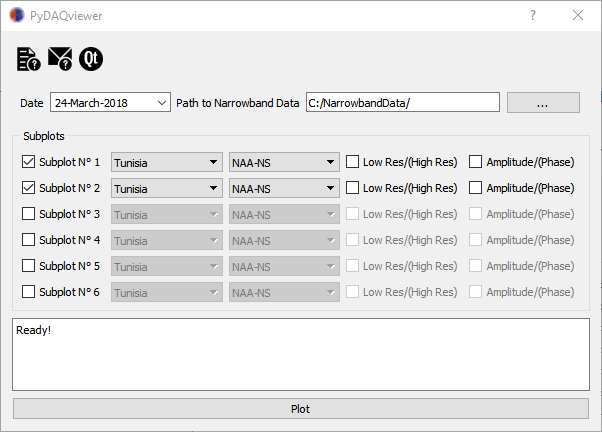
\includegraphics[width=1.0\linewidth]{imgs/GUI_PyDAQviewer.png}}
  \caption{
  PyDAQviewer GUI after running the PyDAQviewer.py script. \label{fig:GUI}
  }
\end{figure}
%\clearpage % flush figures fig:GUI





\begin{figure}[!ht]  % fig:SelectFolder
  \centerline{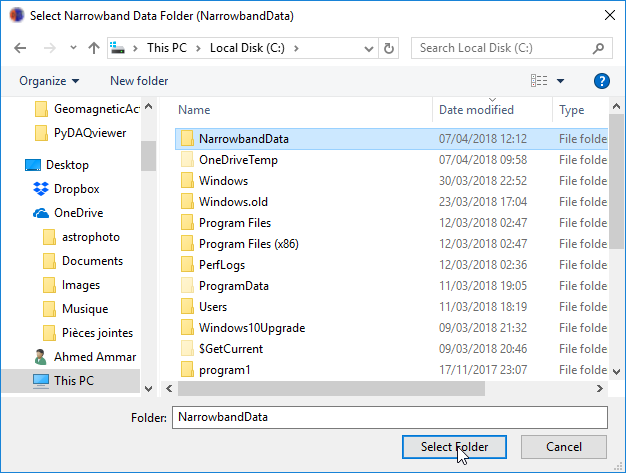
\includegraphics[width=1.0\linewidth]{imgs/opendir.png}}
  \caption{
  Select NarrowbandData folder. \label{fig:SelectFolder}
  }
\end{figure}
%\clearpage % flush figures fig:SelectFolder


The path to your data will be something like: \texttt{'C:/NarrowbandData/SiteName/Year/MM/DD/'} (e.g. \texttt{'C:/NarrowbandData/Tunisia/2018/03/25/'}). Note that this can be on any drive root drive: C-Z including DVD drives etc. So if you burn data to a DVD burn it in the same folder and the PyDAQviewer will be able to find them.

% !split
\subsection{Select date from calander}
After locating the working directory, the user can select AWESOME's data recording date by using a calendar widget as shown in Figure~\ref{fig:SelectDate}.


\begin{figure}[!ht]  % fig:SelectDate
  \centerline{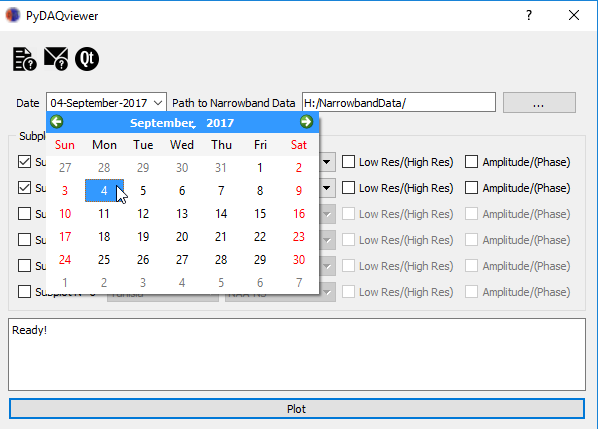
\includegraphics[width=1.0\linewidth]{imgs/SelectDate_PyDAQviewer.png}}
  \caption{
  Select date of the recorded data from the calendar. \label{fig:SelectDate}
  }
\end{figure}
%\clearpage % flush figures fig:SelectDate


% !split
\subsection{Receiver-Transmitter Information}
This file is simply a Python file (Source code below: \texttt{SiteInfo.py}) in which you will enter two dictionaries. The first one is Rx_ID indicating the AWESOME receiver locations and their IDs. The second dictionary is Tx_ID indicating the VLF transmitter IDs and the orientation of their antennas (e.g.~000 for N/S or 001 for E/W). In this way, it is very easy to add any other receiver and transmitter IDs. Then you can simply select the Rx_ID and Tx_ID of interest via menus as shown in Figures~\ref{fig:SelectRx} and~\ref{fig:SelectTx}.

\begin{cod_vpad}{cbg_blue1}\begin{minted}[fontsize=\fontsize{9pt}{9pt},linenos=false,mathescape,baselinestretch=1.0,fontfamily=tt,xleftmargin=2mm]{text}
# -*- coding: utf-8 -*-
#SiteInfo.py
'''
Purpose: Save VLF Receivers (Rx) and Transmitters (Tx) Info   
'''
# Rx info
Rx_ID = {
            "Tunisia":"TN",
            "Algeria":"AL",
            "France":"FR",
            "Japan":"JP",
            "NewYork":"NY",
            "Boulder":"BO",
            "Cheyenne":"CH",
            "Walsenburg":"WS",
            "LasVegas":"LV",
            
            
            }

# Tx info
Tx_ID = {
            "NAA-NS":"NAA_000", 
            "NAA-EW":"NAA_001",
            "NRK-NS":"NRK_000",
            "NRK-EW":"NRK_001",
            "NLK-NS":"NLK_000",
            "NLK-EW":"NLK_001",
            "NAU-NS":"NAU_000",
            "NAU-EW":"NAU_001",
            "NPM-NS":"NPM_000",
            "NPM-EW":"NPM_001",
            "ICV-NS":"ICV_000",
            "ICV-EW":"ICV_001",
            "NSC-NS":"NSC_000",
            "NSC-EW":"NSC_001",
            "GQD-NS":"GQD_000",
            "GQD-EW":"GQD_001",
            "GBZ-NS":"GBZ_000",
            "GBZ-EW":"GBZ_001",
            "DHO-NS":"DHO_000",
            "DHO-EW":"DHO_001",
            "HWU-NS":"HWU_000",
            "HWU-EW":"HWU_001",
            "JXN-NS":"JXN_000",
            "JXN-EW":"JXN_001",
            "ISR-NS":"ISR_000",
            "ISR-EW":"ISR_001"
            }
\end{minted}
\end{cod_vpad}
\noindent



\begin{figure}[!ht]  % fig:SelectRx
  \centerline{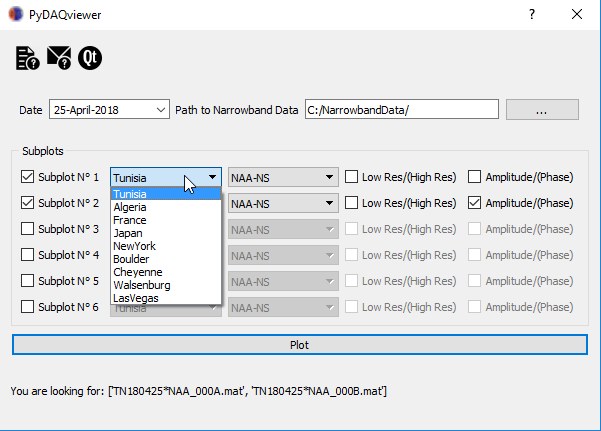
\includegraphics[width=1.0\linewidth]{imgs/SelectRx.png}}
  \caption{
  Select AWESOME station. \label{fig:SelectRx}
  }
\end{figure}
%\clearpage % flush figures fig:SelectRx




\begin{figure}[!ht]  % fig:SelectTx
  \centerline{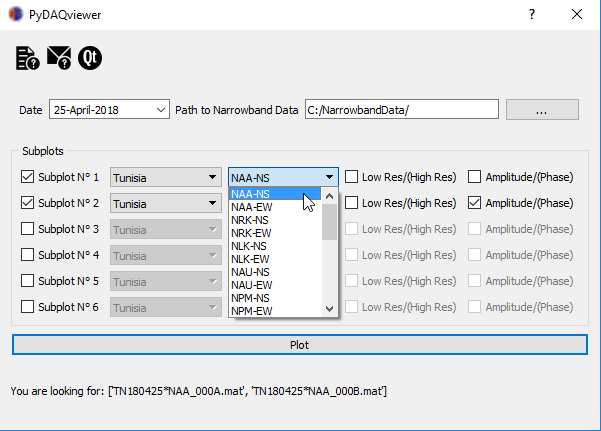
\includegraphics[width=1.0\linewidth]{imgs/SelectTx.png}}
  \caption{
  Select VLF transmitter. \label{fig:SelectTx}
  }
\end{figure}
%\clearpage % flush figures fig:SelectTx



\section{Reproducing the Lightning-Induced Electron Precipitation (LEP) Tutorial}
Now that you have a basic understanding of how the DAQviewer works, it's time to put it to the test and try out all the features. To do this we'll be reproducing a few of the plots you made by hand in the LEP tutorial.

To start edit the \texttt{SiteInfo.py} file to include the Rx_IDs: Cheyenne, Boulder, Walsenburg, and Las Vegas (note in the \texttt{SiteInfo.py} file Las Vegas should be all one word: LasVegas).


\begin{figure}[!ht]  % fig:LEP_Tuto
  \centerline{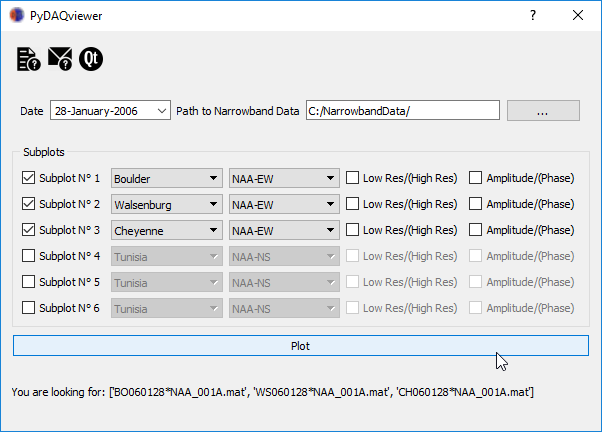
\includegraphics[width=1.0\linewidth]{imgs/LEPtuto.png}}
  \caption{
  Example working on data from LEP tutorial. \label{fig:LEP_Tuto}
  }
\end{figure}
%\clearpage % flush figures fig:LEP_Tuto


The output of this configuration is in below:


\begin{figure}[!ht]  % fig:LEP_figure1
  \centerline{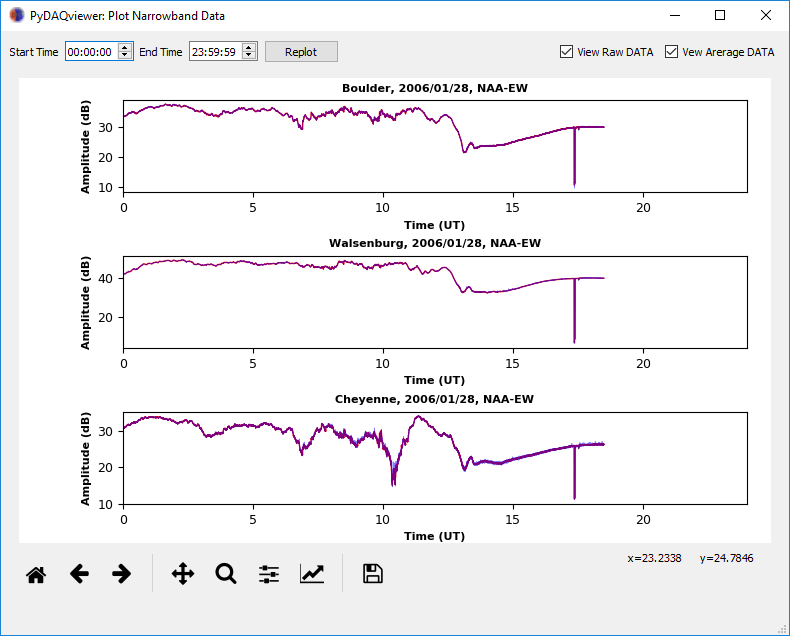
\includegraphics[width=1.0\linewidth]{imgs/LEPfigure1.png}}
  \caption{
  Generated figure. \label{fig:LEP_figure1}
  }
\end{figure}
%\clearpage % flush figures fig:LEP_figure1




\begin{figure}[!ht]  % fig:LEP_figure2
  \centerline{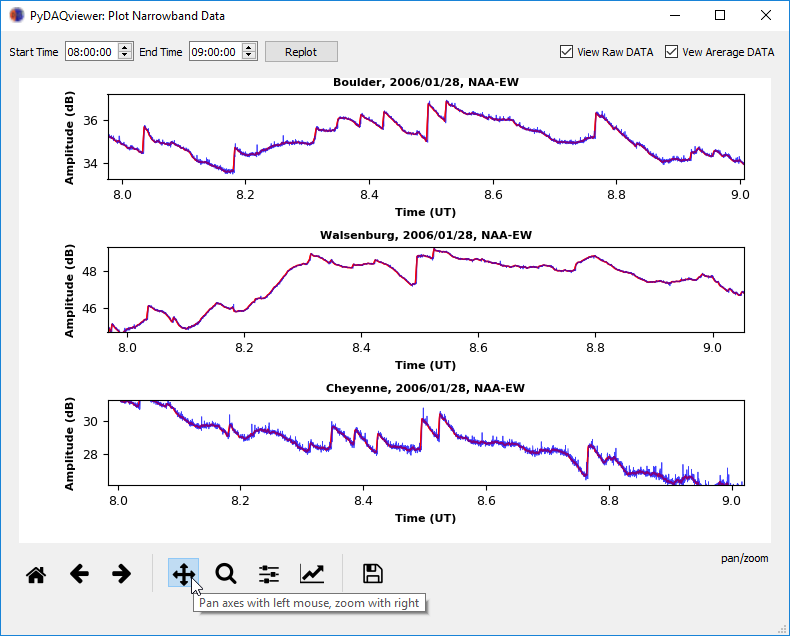
\includegraphics[width=1.0\linewidth]{imgs/LEPfigure2.png}}
  \caption{
  Zoomed figure. \label{fig:LEP_figure2}
  }
\end{figure}
%\clearpage % flush figures fig:LEP_figure2



% ------------------- end of main content ---------------

% #ifdef PREAMBLE
\end{document}
% #endif

